\documentclass{beamer}                             % presentation
% \documentclass[draft]{beamer}                      % improves compile time
\usepackage[utf8]{inputenc}                        % utf8
\usepackage[T1]{fontenc}                           % fix font encoding
\usepackage[english]{babel}                        % language
\usepackage{fvextra}
\usepackage[autostyle, english=american]{csquotes} % quotes
\usepackage{amsmath, amssymb, amsthm}              % ams mathematical packages
\usepackage{physics, mathtools, bm}                % extra math packages
\usepackage{graphicx, subcaption}                  % images
\usepackage{tikz, pgfplots}                        % plots and graphs
\usepackage[cache=true]{minted}                    % source code
\usepackage[style=authoryear-comp]{biblatex}       % bibliography
\usepackage{geometry, hyperref}                    % misc.

\usetikzlibrary{positioning}                       % advanced positioning
\pgfplotsset{compat=newest}                        % version of pgfplots

\graphicspath{{./figures/}}
\addbibresource{references.bib}

%%% math

% serif font in math mode
\usefonttheme[onlymath]{serif}

\newcommand*{\defeq}{\coloneqq}
\newcommand*{\BigO}{\mathcal{O}}
\DeclareMathOperator{\maketen}{make10}

%%% colors

\definecolor{lightblue}{HTML}{a1b4c7}
\definecolor{orange}{HTML}{ea8810}
\definecolor{silver}{HTML}{b0aba8}
\definecolor{rust}{HTML}{b8420f}
\definecolor{seagreen}{HTML}{23553c}

\colorlet{lightsilver}{silver!20!white}
\colorlet{darkorange}{orange!85!black}
\colorlet{darksilver}{silver!85!black}
\colorlet{darklightblue}{lightblue!75!black}
\colorlet{darkrust}{rust!85!black}
\colorlet{darkseagreen}{seagreen!85!black}

\hypersetup{
  colorlinks=true,
  linkcolor=darkrust,
  citecolor=darkseagreen,
  urlcolor=darksilver
}

\setminted[]{
  linenos=true,
  breaklines=true,
  encoding=utf8,
  fontsize=\tiny,
  % frame=lines,
  framesep=2mm
}

\pgfplotsset{compat=newest}
\usepgfplotslibrary{fillbetween}
% make marks not follow the style of lines
\tikzset{every mark/.append style={solid}}
% cache tikz graphics
% \usepgfplotslibrary{external}
% \tikzexternalize
% \tikzsetexternalprefix{external/}

%%% beamer settings

\usetheme{Pittsburgh}
\usecolortheme{orchid}
\usecolortheme{dolphin}

% hide navigation buttons
\setbeamertemplate{navigation symbols}{}
% change title color
\setbeamercolor{title}{fg=darklightblue}
\setbeamercolor{frametitle}{fg=darklightblue}
% table of contents
\setbeamertemplate{section in toc}[default]
% change bibliography entry colors
\setbeamercolor{bibliography entry author}{fg=darklightblue}
\setbeamercolor{bibliography entry note}{fg=lightblue}
% customize \item in itemize
\setbeamercolor{structure}{fg=darklightblue}
\setbeamertemplate{itemize item}{}
\setbeamertemplate{enumerate item}[default]
% enumitem doesn't play well with beamer
% \setitemize{label={},itemsep=0.5cm}
% https://tex.stackexchange.com/questions/16793/
\newenvironment{wideitemize}
  {\itemize\setlength{\itemsep}{0.5cm}}
  {\enditemize}

% title page
\title[]{make10}
\subtitle{}
\author[Huan]{Stephen\ Huan}
\institute[Georgia Institute of Technology]
{
  % Georgia Institute of Technology
  \url{https://cgdct.moe}
}
\date[]{Theory club 2023-09-08}
\subject{Computer science}

\begin{document}
\frame{\titlepage}

\begin{frame}
\frametitle{Overview}
\framesubtitle{}

\tableofcontents
\end{frame}

\section{Introduction}

\begin{frame}
\frametitle{make10}
\framesubtitle{}

\begin{figure}[h!]
  \centering
  
\includegraphics[
    width=0.43\textwidth,
    trim={0 46px 0 650px},
    clip,
  ]{figures/make10.png}%
  
\includegraphics[
    width=0.43\textwidth,
    trim={0 650px 0 0},
    clip,
  ]{figures/make10.png}
  \caption{%
    \href{https://www.takeshobo.co.jp/book_d/shohin/2036201}{%
      \textit{Suugaku Josi}%
    } (\textit{Math Girls}) by Masae Yasuda
  }
\end{figure}
\end{frame}

\begin{frame}
\frametitle{Some examples}
\framesubtitle{}

\begin{exampleblock}{First example}
  2, 4, 6, 8
  \begin{gather*}
    2 + 6 + 8 / 4 = 10
  \end{gather*}
\end{exampleblock}

\begin{exampleblock}{Second example}
  6, 2, 4, 5
  \begin{gather*}
    (6 + 4 - 5) \times 2 = 10
  \end{gather*}
\end{exampleblock}

\begin{exampleblock}{Third example}
  3, 4, 7, 8
\end{exampleblock}
\end{frame}

\begin{frame}
\frametitle{Initial observations}
\framesubtitle{}

\begin{wideitemize}
  \item Easy to prove (just give construction)
  \item Hard to disprove (prove impossible?)
  \item Computer-assisted proofs
  \item Try to prove sequences of numbers can \( \maketen \)
  \end{wideitemize}
\end{frame}

\section{Sequences}

\subsection{Fibonacci}

\begin{frame}
\frametitle{Fibonacci sequence}
\framesubtitle{}

\begin{definition}
  Fibonacci sequence \( F_n \) defined recursively:
  \begin{align*}
    F_0 &\defeq 0 \\
    F_1 &\defeq 1 \\
    F_n &= F_{n - 1} + F_{n - 2}.
  \end{align*}
  The first few terms are \( 0, 1, 1, 2, 3, 5, 8, 13, \dotsc \)
\end{definition}
\end{frame}

\begin{frame}
\frametitle{A claim}
\framesubtitle{}

\begin{theorem}
  \( \maketen([ F_i ]_{i = 1}^n) \) if and only if \( n > 3 \).
\end{theorem}
\only<2->{
  \begin{proof}
    \only<2>{
      \enquote{Base} cases:
      \begin{itemize}
        \item \( n = 0 \): \( \emptyset \).
        \item \( n = 1 \): \( 1 \).
        \item \( n = 2 \): \( 1, 1 \).
        \item \( n = 3 \): \( 1, 1, 2 \).
      \end{itemize}
      All impossible.
      \let\qedsymbol\relax
    }
    \only<3>{
      Base cases:
      \begin{itemize}
        \item \( n = 4 \): \( 1, 1, 2, 3. \)
          \[ (1 + 1 + 3) \times 2. \]
        \item \( n = 5 \): \( 1, 1, 2, 3, 5. \)
          \[ (3 - 2) \times 5 \times (1 + 1). \]
        \item \( n = 6 \): \( 1, 1, 2, 3, 5, 8. \)
          \[ 1 + 1 + 2 + 3 - 5 + 8. \]
      \end{itemize}
      Found contiguous \( n \equiv 1, 2, 0 \pmod 3 \).
      \let\qedsymbol\relax
    }
    \only<4>{
      By induction.

      Let \( n = 3k + r \) for \( k > 1 \), \( 0 \leq r < 3 \).

      By definition \( F_{n + 2} = F_{n + 1} + F_{n}
      \), so \( F_{n + 2} - F_{n + 1} - F_n = 0 \).

      Take { \small \[
        [F_{n + 2} - F_{n + 1} - F_n]
        + [F_{n - 1} - F_{n - 2} - F_{n - 3}]
        + \dotsb + \maketen([ F_i ]_{i = 1}^{k \in \{ 4, 5, 6 \}})
      \] }
      depending on \( r \) (pick \( k \equiv r \pmod 3 \)).
    }
  \end{proof}
}
\end{frame}

\begin{frame}
\frametitle{Commentary}
\framesubtitle{}

\begin{wideitemize}
  \item How reliant on structure was the result?
  \item How far can we push this?
  \item \( F_n \sim \phi^n \) where \( \phi
    \defeq (1 + \sqrt{5})/2 \) is the golden ratio
  \item First prove (surprisingly) useful lemma\ldots
\end{wideitemize}
\end{frame}

\subsection{Constant}

\begin{frame}
\frametitle{Constant}
\framesubtitle{}

\begin{lemma}
  For any integer \( x \neq 0 \), \(
  \maketen([ x ]_{i = 1}^n) \) if \( n > 8 \).
\end{lemma}
\only<2->{
  \begin{proof}
    \only<2>{
      Follow previous sketch.
      \begin{itemize}
        \item \( n = 9 \):
          \begin{align*}
            (x + x) \times (x + x + x + x + x) / x / x
            = (2x)(5x)/x^2
            = 10
          \end{align*}
        \item \( n = 10 \):
          \begin{align*}
            (x / x + x / x) \times (x + x + x + x + x) / x
            = (2)(5x)/x
            = 10
          \end{align*}
      \end{itemize}
      Continuous in \( \pmod 2 \).
      \let\qedsymbol\relax
    }
    \only<3->{
      By induction again.

      Take \(
        (x - x) + (x - x) + \dotsb
        + \maketen([ x ]_{i = 1}^{k \in \{ 9, 10 \}})
      \).
    }
  \end{proof}
}
\only<4>{
  \begin{block}{Conjecture.}
    There exists a constant \( X \) such that for all \( x > X \),
    \( \maketen([ x ]_{i = 1}^n) \) if and only if \( n > 8 \).
  \end{block}
}
\end{frame}

\subsection{Exponential}

\begin{frame}
\frametitle{Exponential}
\framesubtitle{}

\begin{corollary}
  For any integer \( x \neq 0 \), \( \maketen([
  x^i ]_{i = 1}^n) \) if \( n > 16 \).
\end{corollary}
\only<2->{
  \begin{proof}
    Take adjacent quotients of pairs of \(
    [x, x^2, ..., x^n] \), from right to left.

    Let \( n = 2k \) or \( 2k + 1 \) depending on parity of \( n \).

    We get \( [x, ..., x] \), a list of \( k \) or \( (k
    + 1) \) \( x \)'s depending on parity of \( n \).

    But we know \( \maketen \) of a list of \(
    k \) constants is possible if \( k > 8 \).

    So we need \( k > 8 \) or \( n > 16 \).
  \end{proof}
}
\end{frame}

\subsection{Linear}

\begin{frame}
\frametitle{Linear}
\framesubtitle{}

\begin{corollary}
  \( \maketen([ i ]_{i = 1}^n) \) if \( n > 16 \).
\end{corollary}
\only<2->{
  \begin{proof}
    Take adjacent differences of pairs of \(
    [1, 2, \dotsc, n] \), from right to left.

    The proof follows identically, with \( x = 1 \).
  \end{proof}
}
\only<3>{
  \begin{block}{Note.}
    Since \( x = 1 \), it's possible to sharpen the lemma to
    \begin{itemize}
      \item \( n = 7 \): \( (1 + 1) \times (1 + 1 + 1 + 1 + 1) \).
      \item \( n = 8 \): \( (1 + 1) \times (1 + 1 + 1 + 1 + 1) \times 1 \).
    \end{itemize}
    This means we can improve the bound to \( k > 7 \), or \( n > 14 \).

    This is still not even close to tight.
  \end{block}
}
\end{frame}

\begin{frame}
\frametitle{Optimal linear}
\framesubtitle{}

\begin{theorem}
  \( \maketen([ i ]_{i = 1}^n) \) if and only if \( n > 3 \).
\end{theorem}
\only<2->{
  \begin{proof}
    \only<2>{
      Base cases:
      \begin{itemize}
        \item \( n = 1 \). Impossible.
        \item \( n = 2 \). Impossible.
        \item \( n = 3 \). Impossible.
        \item \( n = 4 \). \( 1 + 2 + 3 + 4 \).
        \item \( n = 5 \). \( (1 + 2 + 3 - 4) \times 5 \).
        \item \( n = 6 \). \( (6 - 5) \times (1 + 2 + 3 + 4) \).
      \end{itemize}
      \let\qedsymbol\relax
    }
    \only<3>{
      For \( n > 6 \) consider:
      \[
        [(n - 3) - (n - 1)] \times \left [
        \frac{1 + 2 + \dotsb + (n - 6)}{n - 5} + (n - 4) - (n - 2)
        \right ] + n
      \]
      Clearly every number from \( 1, \dotsc, n \) is included. Simplifying,
      \begin{align*}
        &= (-2)[((n - 6)(n - 5)/2)/(n - 5) - 2] + n \\
        % &= (-2)[(n - 6)/2 - 2] + n \\
        &= -(n - 6) + 4 + n \\
        % &= -n + 6 + 4 + n \\
        &= 10
      \end{align*}
      which was to be proven.
    }
  \end{proof}
}
\end{frame}

\subsection{Polynomial}

\begin{frame}
\frametitle{Towards arbitrary polynomials}
\framesubtitle{}

\begin{wideitemize}
  \item We would like to strengthen this result
  \item Most natural generalization to monomials \( i^k \)
  \item Would like to prove something of the flavor
\end{wideitemize}
\begin{theorem}
  For any natural \( k \) there exists a \( N \) such that
  for all \( n > N \), \( \maketen([ i^k ]_{i = 1}^n)
  \). (Note that \( N \) is allowed to depend on \( k \).)
\end{theorem}
\end{frame}

\begin{frame}
\frametitle{Discrete calculus}
\framesubtitle{}

\begin{definition}
  The \emph{discrete derivative} of a sequence of \( n \) numbers \( f: \{ 1,
  \dotsc, n \} \to \mathbb{R} \) is the new sequence of \( n - 1 \) numbers
  defined by \( \dd f(i) \defeq f(i + 1) - f(i) \) for \( 1 \leq i < n \).
\end{definition}
\begin{theorem}
  \( \dd \) is a linear operator on \( f \).
\end{theorem}
\begin{lemma}
  Recall an operator \( \dd \) is said to be linear if
  \begin{align*}
    \dd(f + g) &= \dd f + \dd g \\
    \dd(c f) &= c (\dd f)
  \end{align*}
  for all \( f, g \in \mathbb{R}^n \) and \( c \in \mathbb{R} \).
\end{lemma}
\end{frame}

\begin{frame}
\frametitle{Derivative of a monomial}
\framesubtitle{}

\begin{lemma}
  If \( f(i) = c i^k \) for some natural \( k \) and real
  \( c \), then \( \dd f \) is a \( (k - 1) \)-degree
  polynomial in \( i \) with leading coefficient \( k c \).
\end{lemma}
\only<2->{
  \begin{proof}
    Use the binomial theorem
    \begin{align*}
      (i + 1)^k
      &= \sum_{j = 0}^k \binom{k}{j} i^j 1^{k - j}
      = \sum_{j = 0}^k \binom{k}{j} i^j. \\
      \dd f(i) &= c [(i + 1)^k - i^k]
      = c \sum_{j = 0}^{k - 1} \binom{k}{j} i^j.
    \end{align*}
    where we used that when \( j = k \), \( \binom{k}{k} i^k = i^k \).

    The leading term is \( c \binom{k}{k - 1}
    i^{k - 1} = c k i^{k - 1} \) as claimed.
  \end{proof}
}
\end{frame}

\begin{frame}
\frametitle{Derivative of a polynomial}
\framesubtitle{}

\begin{lemma}
  If \( f(i) \) is a \( k \)-degree polynomial in \( i \) with
  leading coefficient \( c \), then \( \dd f \) is a \( (k - 1)
  \)-degree polynomial in \( i \) with leading coefficient \( k c \).
\end{lemma}
\only<2->{
  \begin{proof}
    Apply the previous lemma term-by-term with the linearity of \( \dd \).

    For all terms \( i^j \) with \( j < k
    \), derivative has power \( < k - 1 \).

    Thus the only term which affects the leading coefficient
    is \( i^k \), by the previous lemma, derivative
    has leading term \( c k i^{k - 1} \), as claimed.
  \end{proof}
}
\end{frame}

\begin{frame}
\frametitle{Repeated derivatives}
\framesubtitle{}

\begin{lemma}
  If \( f(i) = c i^k \) for natural \( k \)
  and real \( c \), then \( \dd^k f = k ! \).
\end{lemma}
\only<2->{
  \begin{proof}
    Repeatedly apply the previous lemma until left with a constant.
  \end{proof}
}
\end{frame}

\begin{frame}
\frametitle{Proving the claim}
\framesubtitle{}

\begin{theorem}
  For any natural \( k \) there exists a \( N \) such that
  for all \( n > N \), \( \maketen([ i^k ]_{i = 1}^n) \).
\end{theorem}
\only<2>{
  \begin{definition}
    Define the operator \( \dd_2 f \) on \( f \in \mathbb{R}^n \) as
    \[
      \dd_2 f(i) \defeq \begin{cases}
        \dd f[\text{begin} : 2 : \text{end}] & n \equiv 0 \pmod 2 \\
        [f[\text{begin}], \dd f[\text{begin} + 1: 2 : \text{end}]]
          & n \equiv 1 \pmod 2
      \end{cases}
    \]
    in \texttt{Julia} slice notation.
  \end{definition}
}
\only<3->{
  \begin{proof}
    \only<3>{
      Since \( \dd f \) is a \( (k - 1) \)-degree polynomial, \(
      \dd_2 f \) is a also a \( (k - 1) \)-degree polynomial,
      possibly with a \enquote{Dirac} at the beginning.
      \begin{alertblock}{Derivatives of Diracs}
        The derivative of a Dirac at \( i = 1 \) stays a Dirac (with
        flipped sign). This is not true for a Dirac placed in the middle!
      \end{alertblock}
      We can essentially ignore the effect of the Dirac (linearity).
      \let\qedsymbol\relax
    }
    \only<4>{
      Note that \( \abs{\dd f(i)} \leq \abs{f(i + 1)} + \abs{f(i)} \).

      Since each value is represented exactly
      once in \( \dd_2 \), \( \norm{\dd_2 f}_1 \leq \norm{f}_1 \).

      By induction, \( \norm{\dd_2^k f}_1 \leq \norm{f}_1 \), so \(
      \abs{\delta} \leq \abs{1^k + \dotsb + n^k} < \BigO(n^{k + 1})
      \) where \( \abs{\delta} \) denotes the size of the Dirac.

      If we have \( [x, \dotsc, x, y] \), we can
      trivially do this in \( \BigO(\abs{y}) \) \( x \)'s
      by \[ y - [x / x + x / x + \dotsb + x / x]. \]

      Since \( \abs{\delta} \) grows with \( n \), this
      leads to infinite regress (we need more terms to
      control the Dirac, which leads to the Dirac growing).
      \let\qedsymbol\relax
    }
    \only<5>{
      We can get out of this by either finding a tighter
      bound on \( \abs{\delta} \) or a more efficient
      algorithm for controlling the Dirac. We will do both.

      Write \( y \) in binary. Form 2 by \( (x + x) / x \), to get \( 2^i
      \) we need \( i \) copies. For \( i \) digits, need \( \BigO(i^2)
      \) \( x \)'s or \( \BigO(\log^2(\abs{y})) \). Is this enough?

      We can take \( n > \BigO(2^{(1 + o(1)) k}) \). But we can do better.

      We can bound \( \abs{\dd_2^k f(i)} \leq 2^{\binom{k}{2}} k! \). Since
      this is independent of \( n \), we can take \( n > \BigO(2^{k^2}) \)
      which is massive, but workable. With the more efficient algorithm, we
      can take \( n > \BigO(k^2 2^k) \).
    }
  \end{proof}
}
\end{frame}

\begin{frame}
\frametitle{Expressivity of polynomials}
\framesubtitle{}

\begin{theorem}{(Expressivity of polynomials)}
  For any sequence \( f \) on \( n \) terms, there exists a \( (n
  - 1) \)-degree polynomial \( p \) such that \( f(i) = p(i) \).
\end{theorem}
\begin{proof}
  Each \( i \) defines a linear constraint
  in the \( n \) coefficients of \( p \).

  There are \( n \) points and \( n \) coefficients
  defining a \( n \times n \) linear system.

  This system is solvable if and only if all of the points
  (the \( i \)'s) are distinct, which they necessarily are.
\end{proof}
\end{frame}

\begin{frame}
\frametitle{Commentary}
\framesubtitle{}

\begin{wideitemize}
  \item Certificate requires \( \widetilde{\BigO}(2^k)
    \) terms for a \( k \)-degree polynomial
  \item We'd need \( \widetilde{\BigO}(2^n) \)
    terms for an arbitrary sequence of length \( n \)
  \item Trade-off between \enquote{complexity} of sequence (as measured
    by polynomial degree) and \enquote{training data} (number of terms)
  \item From this perspective, \( \maketen \) measures the difficulty
    of the learning problem in modeling/understanding the sequence.
\end{wideitemize}
\end{frame}

\section{Conjectures}

\begin{frame}
\frametitle{Conjectures}
\framesubtitle{}

\begin{block}{conjecture}
  \( \maketen([F_{n}, F_{n + 1}, F_{n + 2},
  F_{n + 3}]) \) is impossible for \( n > 5 \).
\end{block}

\begin{block}{conjecture}
  \( \maketen([n, n, n, n]) \) is impossible for \( n > 20 \).

  (checked by computer up to \( n = 10^5 \))
\end{block}

\begin{block}{conjecture}
  \( \maketen([n, n + 1, n + 2, n + 3]) \) is impossible for \( n > 22 \).

  (checked by computer up to \( n = 10^5 \))
\end{block}

\begin{block}{conjecture}
  For any natural \( k \) there exists a \( N \) such that for all \( n > N
  \), \( \maketen([n^k, (n + 1)^k, (n + 2)^k, (n + 3)^k]) \) is impossible.
\end{block}
\end{frame}

\section{Conclusion}

\begin{frame}
\frametitle{Conclusion}
\framesubtitle{}

\begin{wideitemize}
  \item Children's game to improve mental arithmetic
  \item Study how to \( \maketen \) with longer sequences
  \item How to prove \( \maketen \) is impossible?
  \item Computer-assisted proofs
\end{wideitemize}
\end{frame}

\begin{frame}
\frametitle{Just now...!!?}
\framesubtitle{}

\begin{figure}[h!]
  \centering
  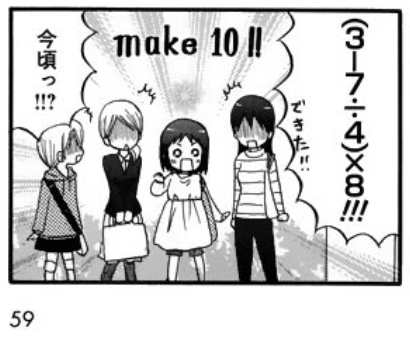
\includegraphics[width=0.75\textwidth]{figures/imagoro.png}
\end{figure}
\end{frame}

\begin{frame}[fragile,allowframebreaks]
\frametitle{Julia code}
\framesubtitle{}
\begin{minted}{julia}
import Base.show


const RATIONAL = false

divide(x, y) = RATIONAL ? x // y : x / y

const OPERATORS = [
    ((x, y) -> x + y, '+', false),
    ((x, y) -> x - y, '-', false),
    ((x, y) -> y - x, '-', true),
    ((x, y) -> x * y, '*', false),
    ((x, y) -> divide(x, y), '/', false),
    ((x, y) -> divide(y, x), '/', true),
]

const LEAF = '.'


struct Tree{T}
    value::T
    left::Union{Tree{T},Nothing}
    right::Union{Tree{T},Nothing}
    name::Char
end


Tree(x) = Tree(divide(x, one(x)), nothing, nothing, LEAF)

isleaf(x) = x.name == LEAF

isunit(x) = !in(x.name, ['+', '-'])

const PAREN_TABLE = Dict(
    '+' => Pair((_) -> true, (_) -> true),
    '-' => Pair((_) -> true, isunit),
    '*' => Pair(isunit, isunit),
    '/' => Pair(isunit, isleaf),
)

function show(io::IO, tree::Tree)
    value = if isleaf(tree)
        Int(tree.value)
    else
        left = repr(tree.left; context=io)
        right = repr(tree.right; context=io)
        left_paren, right_paren = PAREN_TABLE[tree.name]
        left_repr = !left_paren(tree.left) ? "($left)" : left
        right_repr = !right_paren(tree.right) ? "($right)" : right
        "$left_repr $(tree.name) $right_repr"
    end
    return print(io, value)
end


function key(nums)
    return Tuple(sort([tree.value for tree in nums]))
end

make10(nums) = make10!(collect(map(Tree, nums)))

function make10!(nums; cache=Set())
    n = length(nums)
    n == 0 && return nothing
    n == 1 && nums[begin].value == 10 && return nums[begin]
    for i in 1:n
        for j in i:(n - 1)
            for (op, name, flip) in OPERATORS
                x = popat!(nums, i)
                y = popat!(nums, j)
                value = op(x.value, y.value)
                pushfirst!(nums, Tree(value, flip ? y : x, flip ? x : y, name))
                k = key(nums)
                if !in(k, cache)
                    push!(cache, k)
                    rtn = make10!(nums; cache)
                    # no need to maintain the invariant
                    !isnothing(rtn) && return rtn
                end
                # restore order
                popfirst!(nums)
                insert!(nums, j, y)
                insert!(nums, i, x)
            end
        end
    end
end

@assert !isnothing(make10([2, 4, 6, 8])) "failed example 1"
@assert !isnothing(make10([6, 2, 4, 5])) "failed example 2"
println(make10([3, 4, 7, 8]))
\end{minted}
\end{frame}

% \printbibliography
\end{document}
